% This will be the main document for the Technical Networks paper to
% be written by the Eggnet team of Jordan Ell, Triet Huynh and Braden
% Simpson in association with Adrian Schroeter and Daniela Damian.

\documentclass[conference]{IEEEtran}

% Use of outside images
\usepackage{graphicx} 
% Use text inside euqations
\usepackage{amsmath}

\usepackage{float}
\floatstyle{plaintop}
\restylefloat{table}

% Correct bad hyphenation here
\hyphenation{op-tical net-works semi-conduc-tor}

% Begin the paper here
\begin{document}


% Paper title
% Can use linebreaks \\ within to get better formatting as desired
\title{Automatic Elicitation of Requirements From Internet Forums With Forum Miner}

% Authors names
\author{\IEEEauthorblockN{Jordan Ell}
\IEEEauthorblockA{University of Victoria,
Victoria, British Columbia, Canada \\ jell@uvic.ca}
}

% Make the title area
\maketitle


\begin{abstract}
Internet forums are a great application for talking about your favorite piece of software
or even a video game. However, forums themselves do not provide the ability to perform any sort
of deep analytical queries on their information. We cannot easily extract what stakeholders
are talking about and how that discussion can be turned into new requirements for the software
system. The best that we currently have as an industry
are community managers, who monitor online forums and report back to developers for improvement
suggestions. This manual process is why I have created the tool known as ``Forum-Miner'' which
is a forum analytical tool for Blizzard Entertainment game forums to determine what players are talking about
and how those conversations can be used to improve the game through new requirements. Through the use of web crawling,
big data, and natural language processing, I have created an easy to use website for deep forum analytics 
which provides visualization and aggregation of player thoughts while current requirement detection
remains under heavy development and prototyping.
\end{abstract}


\section{Introduction}
Internet forums are a great place for stakeholders of a software project to communicate and discuss the
project at hand~\cite{Elsas:2010:STF}. While some forums can be more existential discussion based, many forums have a feedback
or review topic section which allows users to talk about possible improvements to the software, possible
changes they wish to see made, or even bug fixes. A software focused forum may also have unique topics
such as feature discussion where stakeholders can discuss the single feature.
Inside any given forum topic, threads are created. Threads are created by an individual wishing to express
some idea or opinion. This thread is usually accompanied with a title and some initial body text. Once
a thread is created, other users can post comments inside the thread as per the thread's topic and direction
with plain body text replies. One of the largest cases where we can see 
a community of stakeholders come together to discuss ideas of software are in the Internet forums of video games.

Blizzard Entertainment~\footnote{http://us.blizzard.com/en-us/} is a great example of how Internet forums
can be used to discuss new features of video games as well as discuss patches, existing features and
how the games should move into the future. We know that Blizzard Internet data has been used
to improve game play before~\cite{Lewis:2010:MGS}, but can we take the information in the online forums
to improve the game specifically? The issue with these online forums however, is that their size
is quite daunting~\cite{Glance:2005:DMI}. If for example, we look at the Blizzard forums, we see that for each of their 5 games,
thousands and millions of threads have been created and discussed. In order to analyze these threads as
per developer and business needs, we so far only have human intervention. If we look at the Blizzard online job
postings~\footnote{http://us.blizzard.com/en-us/company/careers/posting.html?id=13000DX}, 
we can see that they hire ``Community Managers'' which are in charge of sorting through the thousands
of threads in order to see what players are actually talking about online. This manual sorting turns into
new requirements that are passed to project managers and possibly implemented by developers. This is a terribly
inefficient system.

From previous works, we know that natural language processing, while it can pose many problems in filtering
content~\cite{Chandy:2012:ISI} and creating exact machine readable representations of what is said~\cite{Abney:1996:PST},
can lead us down the correct path. Many previous researchers have had successes data mining online reviews of
products (mostly in app stores) to find out what features are being talked about~\cite{Pagano:2013:FAS} and
how the discussions can relate to software success~\cite{Dave:2003:MPG}. Through leveraging some of these previous
techniques, I wish to create a methodology which can address the gap of the ``Community Manager'' human input
by automatically eliciting new requirements for a software system from pure text feedback from end users.

This paper shows a way in which we can monitor online forums for Blizzard's video games in an automatic fashion
and provide developers with the information that they need for new requirements. To achieve this, I created a website
tool called Forum-Miner (FM), which by using natural language processing techniques, is able to sort
through thousands if not millions of forum threads and identify trend in conversation in both volume and sentiment
as well as provide developers with new requirements to the particular game that fits with the end user's goals.

The rest of this paper is laid out as follows. Section ~\ref{sec:related} will go over the related work to 
the methodologies and results of this paper. Section~\ref{sec:meth} will outline the technical details
of how the website was made and how it can be used by end users. Section~\ref{sec:eval} will go over
my evaluation of the FM tool. Section~\ref{sec:fw} will outline
the future work that is planned for this website and how it will change over time to better support
deeper analysis of the Blizzard forums. Finally, ~\ref{sec:conc} will give a final conclusion of what has 
been learned over the course of this project.

\begin{figure*}[tb!]
\centering
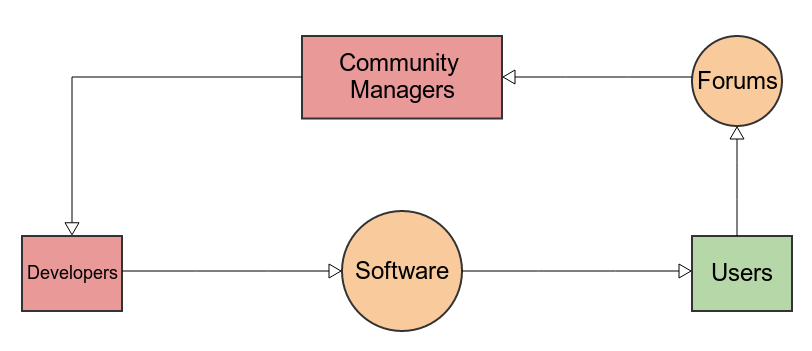
\includegraphics[width=0.7\textwidth, height=150px]{images/requirements.png}
\caption{A typical requirements flow chart with human intervention.\label{fig:requirements1}}
\end{figure*}

\section{Related Work}
\label{sec:related}

Since many software requirements are identified only after a product has been released for public
or end user use, much research has been made to automatically elicit those requirements from the
users through various feedback mediums. One particularly well studied feedback system is that of
Mobile device application stores and their user feedback pages.

Pagano et al.~\cite{Pagano:2013:FAS} performed an empirical study on user feedback in the Apple
App Store. They mainly discussed the usage of user feedback by the users, the content of the user
feedback and its impact on the user community in the App Store. They performed this analysis by
utilizing some statistical approaches. Pagano et al. found that most crucial and most feedback
in terms of volume is submitted directly after a major release of an app. This understanding
is crucial to understand when the most relevant feedback will be given by a user. This information
could also be paired with software patch note analysis to see what was changed in a release and
how users responded in their feedback. Pagano et al. also found that developers can and should
use the App Store reviews to better their product and that users frequently share their needs,
ideas, and experience in their reviews which is exactly what requirements elicitation requires.

Being able to identify legitimate feedback versus spam is also a large consideration to consider
when eliciting requirements automatically from Internet feedback. Chandy et al.~\cite{Chandy:2012:ISI}
have created a classification system for the identification of spam in the Apple App Store. The authors
present a model which is able to classify apps, developers, users, and more importantly, reviews into
normal or malicious categories. Since we know from studies that malicious reviews or text can often
impact the success of an app on the Apple App Store~\cite{Pagano:2013:FAS} it is important to be
able to filter these types of reviews, or in the case of this paper, malicious text, from the algorithms
which will determine qualities of the text or software. Since Internet forums can often contain
malicious or ill intended content, this filtering of data is a crucial step in gathering requirements
automatically and having a low false positive rate.

Finkelstein et al.~\cite{Finkelstein:2013:MAS} introduced a method to extract feature
and price information of the applications available on the Blackberry App Store which
is used to predict prices of the apps. While the prediction of price of software does not directly
correlate to the research being conducted in this paper, the feature extraction does. If we know
what features are put into a product, we can make better implications about what is being
discussed in Internet forums and how it relates to the product. For our purposes, patch notes
could suffice to allow this type of feature extraction of the software being studied. We will
know what feature the software has as well as what has been changed lately to better inform
our decision making from the Internet forum parsing.

As far as natural language processing for requirements elicitation, 
parts of speech tagging~\footnote{http://en.wikipedia.org/wiki/Part-of-speech\_tagging} has
become quite a prevalent step in understanding natural language and deciphering exactly
what users are talking about as per requirements needs. Parts of speech tagging involves marking 
each word in a group of works (a sentence for example) as corresponding to a particular part of speech
based on its definition as well as its context of surrounding words. These groups of tags can then be
machine processes in order to discover what is needed from the sentence in terms of its structure
and components for the requirements gathering process.

In terms of the strengths of parts of speech tagging, Abney~\cite{Abney:1996:PST} shows how
the disambiguation of speech such as ``give John help'' versus ``let John help'' can be quite
troublesome and that an exact solution may be far beyond reach. However, Abney shows that a
reasonable approximate solution is quite feasible using the ideas of partial parsing. Partial
parsing involves starting by tagging all possible words in a sentence and then building
possible relations between those words based on a grammar like structure in the words. An
iterative method is applied to the tags in order to build up whole structures in the sentence
or group of words that can disambiguate example such as the aforementioned with helping John.
Being able to disambiguate examples such as helping John is a very crucial step when it comes
to eliciting requirements from online text forums.

Abney continued his word on parsing of natural language with tagging through the use of
finite state cascades~\cite{Abney:1996:PSC}. Finite state cascades consists of a series of finite
transduction where a set of adjacent tags in a group of words can be transformed into a higher
level tag or tags. These transductions can be repeated as necessary until no more are possible
or the initial tag searcher for is found. This is an extremely important research topic to consider
when extracting requirements from free text. For example, requirements can be often broken into an
object and a verb phrase associated with the object. The object can usually be found by simple
parts of speech tagging but the verb phrase is often built from many different parts
of speech and can be accomplished through this finite state cascades methodology. Examples of 
finite state cascades can be seen in Figure~\ref{fig:parsing} and Figure~\ref{fig:rules}

Hu et al.~\cite{Hu:2004:MSC} present their methodology for summarizing customer reviews from the 
Internet for various products. Their methodology consists of three steps: mining for product
features that are being discussed positively or negatively, identifying opinions of features
and classifying them positive or negative, and finally, summarizing the results. Hu et al. use
parts of speech tagging  in order to identify the most
frequent features of the product being talked about, then use sentiment analysis to find how
users feel about said feature. This paper represents the possibilities for automatic requirements
elicitation through the use of parts of speech tagging and feature extraction. As will be seen
later in the paper, I use nouns as well as objects of sentences (as per Hu et al.) to identify
features. Further study and comparisons of these models may be needed.

There has also been a considerable amount of research put forward for sentiment analysis of
text from the Internet. Dave et al.~\cite{Dave:2003:MPG} were among the first researchers
to look at the job of classifying reviews of a product online into either positive or negative.
Their model relies heavily on information retrieval techniques for feature extraction and scoring
of those features based on context of the review. Dave et al. showed how machine learning techniques
can be applied to free text analysis for classification of positive and negative reviews. Not only
does this research tie in with Chandy et al.~\cite{Chandy:2012:ISI} work of potential spam filtering,
but it also provides us with another path for classifying sentiment of features when deriving
requirements. As will be seen, the requirements gathered can rage from extremely positive to
negative changes. It may be useful for a developer to know that users are angry about a feature
when requesting a change or fix to it as opposed to happy with the feature and only suggesting new ideas.

While there have been many successes at requirements gathering after a product has been released,
Ko et al.~\cite{Ko:2011:CSP} found that most constraints when dealing with user feedback emerged
from the diverse use of the application and the assumptions made by end users about the architecture
derived from previous requirements. Ko et al. performed a 6-month case study of a web application for
a university community and studied the bug reports as well as conducted interviews with users and
non-adopters of the system. We can see these problems continue to arise in automatic elicitation of
requirements from text as conflicting view points between multiple users can cause issues and the need
for human intervention as conflicting requirements may be derived.

\begin{figure}[h]
\centering
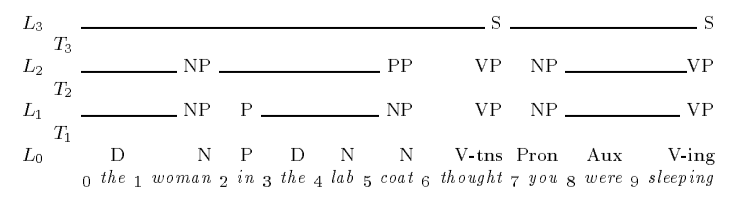
\includegraphics[width=0.5\textwidth]{images/parsing.png}
\caption{A screen shot of activity measure graph.\label{fig:parsing}}
\end{figure}

\begin{figure}[h]
\centering
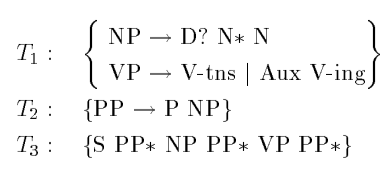
\includegraphics[width=0.5\textwidth]{images/rules.png}
\caption{The transductions to be applied in the parsing from Figure~\ref{fig:parsing}.
\label{fig:rules}}
\end{figure}

\section{Methodology}
\label{sec:meth}

In order to create the website ``Forum-Miner'', several technologies has to be used to create
the unique set of analysis tools which can be seen in the final product. These tools included: Python scripts,
Ruby on Rails web framework, HTML5 technologies, and natural language processing.

\subsection{Collecting Forum Data}

In order to collect forum data from Blizzard, a few steps needed to be taken. First, how to store the forum
data must be considered as it will impact the design decisions of visualization moving into the future. I decided
to store the data in a PostgreSQL database as it allowed me to create the final web application I wanted with
greater ease (through Ruby on Rails) than storing into a NoSQL database or just plain files for Map Reduce jobs.
Second, I had to figure out a way to actually pull the data down from the Blizzard web pages. After doing some
research, I saw that Blizzard had no REST API available for programmers to use on their forums. This being
the case, I resulted to writing a web crawler in Python. I used the Python library called ``BeautifulSoup'' in
order to complete the web crawling. Once data was able to be pulled down, I stored the data in the PostgreSQL 
database with a very simple schema of thread and comments. I omitted the topics of the forum because I wanted
my final product to be generalizable to all online forums, not just those with defined topic areas.

The only major hiccup along the way of pulling down this data was the loss of connections from the web crawler
which could occur while it was running. (I was initially concerned about becoming IP banned by Blizzard for
using up too much bandwidth, but that did not end up being a problem.) So in order to mitigate a connection loss,
I throttled the speed in which I would visit web pages in order to slow down the connection. This resulted in
myself having to run the crawler for longer periods of time to ensure accuracy. However, this also means that
I did not collect all the data available on the forums. In fact, I crawled roughly 75,000 pages from a total
of near a million.

\subsection{Forum Analysis}

This section involves many different analysis techniques. Each technique is associated with a picture from
the resulting web interface.

\subsubsection{Activity}

The activity of the online forums is straight forward. I simply took how many comments were created on each
day for the last year and plotted them on a stock ticker graph using ``HighCharts.js''. This can be seen in
Figure~\ref{fig:activity}. The activity can also be plotted by topic. (Topic identification and search will
be shown later.) Once the user enters in a topic he or she would like to learn more about, the same aggregation
happens, only with a filter on that topic. Only comments which are in the topic provided are counted against
the daily totals on the graph.

\begin{figure}[h]
\centering
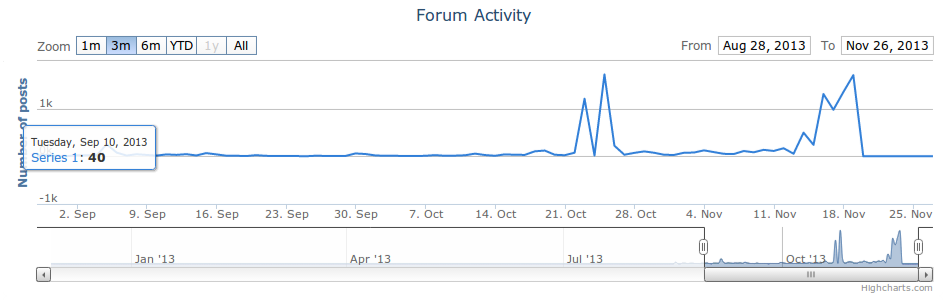
\includegraphics[width=0.5\textwidth]{images/activity.png}
\caption{A screen shot of activity measure graph.\label{fig:activity}}
\end{figure}

Activity can be used to gage the community's response to some event occuring in the ``Blizzard Universe''.
For example, a user of FM could have a list of patches present while using FM (The ability to add patch notes
and dates to FM will come as a later feature) and determine if any large activity spikes occurred directly
after a major release. We know from Hu et al.~\cite{Hu:2004:MSC} that some of the best feedback comes directly
after a major release, so this may be a good starting point for further exploration of user feedback. If an
activity spike is spotted, the user could take it one step further with sentiment analysis to come next.

\subsubsection{Sentiment}

For every comment that came in, every word of the comment was separated in order to analyze them on their own.
Each word was assigned a sentiment score as per the document handed out in this class for assignment 1
known as AFINN-111. This document has a variety of English language words with scores assigned to them
between -5 and +5. If a word is assigned a negative score then that means it has negative sentiment (sad, 
angry, etc.) and if it has a positive score it has a happy sentiment. As per the comments, each word is assigned
a score and the total score for the comment is the aggregation of word scores within the comment. This final
score is also clamped between the values of -5 and +5 to avoid single comments skewing the results of
final analysis techniques. 

The results of the sentiment analysis is shown in Figure~\ref{fig:sent}. If no topic is specified, all comments
are used in the total sentiment analysis. If however, a user uses the search bar to provide a topic, only those
comments containing that topic are used.

\begin{figure}[h]
\centering
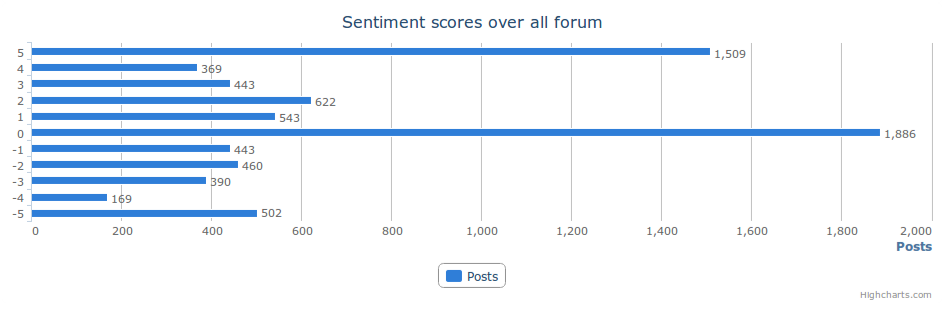
\includegraphics[width=0.5\textwidth]{images/sent.png}
\caption{A screen shot of sentiment measure graph.\label{fig:sent}}
\end{figure}

While sentiment on its own may not be extremely useful, it can be applied to gain context into a particular
topic of the forums. For instance, we may want to examine the game ``Hearthstone'' and in particular the
``Priest'' class that comes as part of the game. If we do a search for ``Priest'' we may find that overall
comments on the forum are quite negative about this particular class. This could be a good indication that
some requirements demanded by the community are not being met by the game developers. On the other side,
if we see that the sentiment is very high for ``Priest'' we might decide that the community is generally 
happy with the class and that developers should focus their efforts elsewhere in the project in order to
better fulfill the requirements from upset users. This sense of sentiment is very important when it comes
to time management of developers on new features. Should the developers focus on fixing old issues, or 
implement new feature to keep users pleased.

\subsubsection{Related Topics}

When a user searches for more information about a particular topic on the forum, FM presents them with related
topics to their search terms. In order to accomplish this, I used the python library called ``Topia''. Topia 
uses Parts of Speech in order to categorize every word from every post as noun, adjective, verb, etc. Once these
categorizations are completed, I simply filtered the words on nouns, objects, and verbs. This subset became the
list of topic words for any given comment. Once these keyword topics had been extracted, it was a simple algorithm
of seeing which keywords are referenced the most with the user provided topic. I ended up limiting it to the
top 50 keywords so as to not overwhelm the user. I found that the top 10 keywords ended up being the same for most
topics provided by the user, but the related topics ranked 10th - 30th were often quite useful. The related topics
can be seen in Figure~\ref{fig:rel}

\begin{figure}[h]
\centering
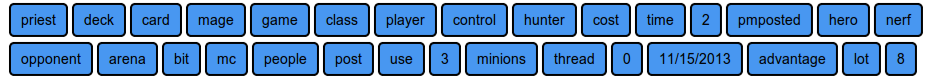
\includegraphics[width=0.5\textwidth]{images/rel.png}
\caption{A screen shot of related topics tags.\label{fig:rel}}
\end{figure}

These lists of related words can be very important into providing more context for the (to come) new requirements.
We might see that a requirement for one object involves the changing of another. So we can detect that this other
object is a related object and we can apply the same analysis to it. We can see its own sentiment, activity and
requirements. A case may arise where a requirement to one object really just requires a change to another. This
type of deeper analysis was not possible before.

\subsubsection{Requirements}

When a user searchers for more information about a particular topic, FM will present a list of requirements
as designated by the community surrounding that topic. In Figured~\ref{fig:req}, we can see that when
the user searchers for the term ``Priest'', objects that are related to the Priest object in the game come up
with their recommended requirements.

\begin{figure}[h]
\centering
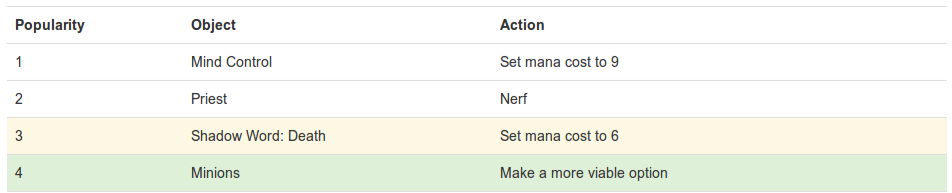
\includegraphics[width=0.5\textwidth]{images/req.png}
\caption{A screen shot of automatically detected requirements through their game object and
requested action.\label{fig:req}}
\end{figure}

The results seen in Figured~\ref{fig:req} are hard coded for this example as the actual algorithm implemented
was not quite as good as was expected (I will address this in Section~\ref{sec:eval}). In order to achieve these
results, I followed the following algorithm. First I found which keywords were related to the search term as
seen in the related topics section above. Once I had these, I found which sentences in which posts correlated
to these topic discussion. I then used ``Topia'' once again in order to label the Parts of Speech found in
the sentences. I then extracted the objects and verb phrases of the sentences. 
Verb phrases were constructed using finite state cascades~\cite{Abney:1996:PSC}. For instance, the sentence 
``I think that Mind Control is too strong and that it should be set to 9 mana.'' will have extracted
Mind Control as the object and set to 9 mana as the verb phrase. This was my initial idea for the requirements
algorithm, however it yielded very difficult to read output and require myself to intervene and make the
results readable, in terms of sentence structure, to other users. I have plans to improve this algorithm
which I will talk about in Section~\ref{sec:fw}.

An important part of this algorithm is the sentiment score that is assigned to each of the requirements
automatically returned to the user. For example, if players a very upset that the ``Priest'' class is too
strong in the game they have have submitted their fix which is to set the ``Mind Contol'' card to a higher
cost than before. This requirement would have a negative sentiment score attached to it because the players
are asking for a fix to some negative aspect of the game in their opinion. This is a very important step
when it comes to analyzing new requirements from a developers stand points. A developer may be more focused
on keep existing user happy by tweaking the game to their opinions rather than adding new features which may
entice new players to join the game. This extra level and analysis takes the requirements to the next step
to allow developers to determine where their priorities are.

\subsection{Visualization}

In order to visualize all of the previous analysis techniques, I used a variety of tools. I first used Ruby
on Rails in order to create a web application to host all of my findings. Ruby on Rails allows for quick prototyping
of website so it was an easy selection for this project. Rails is, obviously, written with a Ruby backend implementation
and contains a full MVC (model view controller) web stack built in.

I next had to find a way to graph both the sentiment and activity analysis I performed. I originally had planned
to use Google Charts as I had used them before in other big data applications, but I actually stumbled across
HighCharts.js, which is a great charting application for big data. HighCharts.js is a native only JavaScript
charting program which only requires jQuery (added in most projects anyways). This lack of dependency made it
an easy tool to work with. HighCharts.js supplies users with two basic charting applications, Chart and StockChart.
For the displaying of the activity I used the StockChart view. The StockChart view allows the user to control
how much data to be viewed by using the built in slider or preset buttons. This was a great choice for the activity
controls as activity can differ drastically from month to month and viewing particular time frames is very useful.
For the sentiment scores, I used the simple Chart template. I chose to show a bar chart to emphasize where the
bulk of sentiment scores lie and for ease of reading. This bar chart also takes into account the amount of activity
to that higher activity rates do not skew the users perception of sentiment. The sentiment charts shows only
the scores from the previous month to date comments.

Finally, for styling purposes, I used Twitter's Bootstrap CSS framework. Bootstrap is used in many web applications
for its ease of use and for its polish.

\section{Evaluation}
\label{sec:eval}

\textit{A note about this evaluation: Since the requirements feature of FM is not completely human readable,
I wanted to test whether or not, given the other contextual information provided by FM in the activity,
sentiment and related topics, a human could interpret the semi readable requirement from having no knowledge
of the software project.}

In order to fully evaluate this tool, I would need to conduct case studies with current ``Community managers'' of
various software products to test if FM makes their lives easier or can provide any sort of assistance to their
day to day jobs. However, I did not have time to conduct such a study, so instead I conducted a very minor study
with a single participant to see what they could learn from the tool versus what I knew from analyzing forum
contents manually.

In this evaluation I had a grad student at the University of Victoria use FM with a particular focus on the
game ``Hearthstone'' and the game class called the ``Priest''. The student's job was to explore the data presented
in FM and come up with any requirements for the ``Priest'' class without having knowledge of the game. I participated
in this study as a knowledgeable observer. If the participant had any questions about objects they were seeing in the
data I would tell them what the object was and how it was used in the game. I did not give any indication as to
any potential requirements that may be needed for such an object.

I had 4 potential requirements that the participant could identify as evaluation criteria. The participant ended
up only identifying 1 of the 4 requirements. The 1 requirements identified was a strong negative sentiment requirement.
This showed that given only a semi human readable requirement, the contextual information provided by FM was enough to
deduce the very strong requirements suggestions by the community. However, this also showed that creating human
readable language for requirements will be needed for any further use of FM.

\section{Future Work}
\label{sec:fw}

For the future work of this project, I really only have one major focus, but due to the nature of web applications,
other interesting additions can be created with ease. My main focus moving forward is in the further development
of the requirements elicitation tool. As per Figure~\ref{fig:req}, we can see how automatically generated
requirements may becomes handy to developers in that they can see what the community wants. However, finding 
these requirements and displaying them in a way that makes sense is difficult as found with this project.

In order to improve the requirements I suggest 2 steps. First to make the results more human readable, I would
like to incorporate other factors of the source sentences aside from object and verb phrase in order to make
the results a more cohesive sentence. Second, I would like to use some of the ideas from plagiarism detection
software and research in order to rank the findings better. Plagiarism research deals with taking two pieces of
English, say two sentences, and determining how alike they are. I would use this idea to find similar requirements.
If I can find requirements that are talked about by 90\% of the community, they are probably more high end priorities
for developers than a single suggestion by one user.

Through these two changes, I hope to make Forum-Miner a more robust tool and to eventual support community manager
jobs for software development.

\section{Conclusions}
\label{sec:conc}

This paper has walked through the creation and implementation of the ``Forum-Miner'' web tool. I have shown
how through the use of Python and web crawling, storage facilities, and Ruby on Rails, how we can create tools
which can perform deep analysis on natural unstructured data
that is available on the web through software system forums. Moving forward, I do not only hope to improve my
website by the better implementation of the requirements gathering algorithm, but I also hope to open the ideas
of this paper to further unstructured data research on the web. Free text is all over the place on the Internet,
but we do not yet have the tools to harness it.

I hope to release ``Forum-Miner'' to a public web server near April 2014 as I will be continuing this project
as a directed studies in the following semester. The code is available on GitHub.

\bibliographystyle{IEEEtran}
\bibliography{paper}


% End of the paper
\end{document}
